\documentclass[12pt]{article}

%%% PAGE DIMENSIONS
\usepackage{geometry} % to change the page dimensions
\geometry{letterpaper} % or letterpaper (US) or a5paper or....
\geometry{margin=1in} % for example, change the margins to 2 inches all round
% \geometry{landscape} % set up the page for landscape

\usepackage{graphicx} % support the \includegraphics command and options

%%% PACKAGES
\usepackage{booktabs} % for much better looking tables
\usepackage{array} % for better arrays (eg matrices) in maths
\usepackage{paralist} % very flexible & customisable lists (eg. enumerate/itemize, etc.)
\usepackage{verbatim} % adds environment for commenting out blocks of text & for better verbatim
\usepackage{float} % for placement of figures 
\usepackage{caption} % make it possible to include more than one captioned figure/table in a single float
\usepackage{subcaption}
\usepackage{xcolor} % provides colors for text (eg. source code color defined in lstset)
\usepackage{listings} % include source code from any programming language
\lstset {
	language=[LaTeX]TeX,
	breaklines=true, 
	frame=single,
	basicstyle=\small, 
	keywordstyle=\color{blue}, 
	commentstyle=\color{red},
}
\usepackage{url} % for neatly displaying the urls of websites
\usepackage[none]{hyphenat} % disable line-wrap hyphenation

% Linguistics packages
\usepackage{tipa} % provides IPA symbols
\usepackage{phonrule} % provides phonological rule framework
\usepackage{qtree} % provides Syntax Trees

% Bibliography Stuff
\usepackage{apacite}

%%% HEADERS & FOOTERS
\usepackage{fancyhdr} % This should be set AFTER setting up the page geometry
\pagestyle{fancy} % options: empty , plain , fancy
\renewcommand{\headrulewidth}{0.0pt} % customise the layout
\lhead{}\chead{}\rhead{\thepage} % define your header, \thepage command provides the page number
\lfoot{}\cfoot{}\rfoot{} % footer

\setlength{\parindent}{4em} % set paragraph indent
\renewcommand{\baselinestretch}{1.5} % set line spacing

\usepackage{gb4e} % provides environment for linguistic examples, tools for glosses, and other goodies

%%% END Article customizations

\title{A Linguist's Guide to Easy Formatting: \\
\large A Crash Course in \LaTeX \vspace{-2ex}}
\author{Neal Digre\thanks{This work was completed, in part, during my coursework for the Computer Science Department at Western Washington University. If you have questions, comments, or suggestions for additional topics you'd like covered, please email me at neal[dot]digre[at]gmail.com} \vspace{-2ex}}
\date{}

\begin{document}
\maketitle
\pagestyle{fancy}

\section{Introduction}

It's only hours until the deadline and your linguistics paper is a jumble of words, diagrams, and fonts. It seems that no amount of cat-herding can fix your formatting woes. Every time you fix one issue another one crops up in its place. With this guide to easy formatting, you can turn even the most chaotic drafts into a clean, polished, professional looking paper that will surely impress your audience and keep those unruly cats at bay.

{\LaTeX} is a \textsc{free} document preparation system that takes away the worry of formatting and lets the author focus on content. {\LaTeX} includes several useful tools that make formatting for linguistics particularly convenient.

We begin by walking through downloading {\LaTeX} and learning a few {\LaTeX} document essentials, like the preamble, sectioning, and figures. Once we have the basics down, we delve into some of the linguistic applications, looking at how to write IPA symbols for phonetics using {\LaTeX}'s \verb!tipa! package. There's also an overview of {\LaTeX}'s Syntax tools, including the creation of syntax tree diagrams with \verb!qtree! and numbered examples with \verb!gb4e!. For more advanced users, I touch briefly on creating a bibliography and appendices. Lastly, if you want to learn more about {\LaTeX}, the web addresses of several documentation pages are provided in Appendix B.

\section{Getting Started} 
\subsection{Installing \LaTeX}

Let's begin by learning how to install {\LaTeX} on your own computer. Go to the {\LaTeX} project site by copying this url, \url{https://latex-project.org/ftp.html}, into your web browser address bar. Then, select the proper version for your operating system, and follow the instructions for downloading the appropriate \verb!.pkg!, \verb!.exe!, or \verb!.zip! file. Once the download finishes, click on the downloaded file to start the installer. Again, follow the on-screen instructions. After that's finished, you're ready to use {\LaTeX}! It's that simple! If you do happen to run into problems with installation, visit {\LaTeX}'s Help section or Google; there's a massive online community of {\LaTeX} users that have probably run into similar issues.

\subsection{Document Basics}

\subsubsection{Commands and the Preamble}

\begin{figure}[h]
\centering
\caption{A preamble example}
\label{fig:preamble}
\begin{tabular}{c}
\begin{lstlisting}
\documentclass[12pt]{article}
\usepackage{geometry} 
\geometry{letterpaper} % change the page dimensions
\geometry{margin=1in} % change the margins
\usepackage{fancyhdr} % Set this AFTER setting up the page geometry
\pagestyle{fancy} % options: empty , plain , fancy
\renewcommand{\headrulewidth}{0.0pt} % customise the layout...
\lhead{}\chead{}\rhead{\thepage} % add a header with page #
\setlength{\parindent}{4em} % set paragraph indent
\renewcommand{\baselinestretch}{1.5} % set line spacing
\end{lstlisting}
\end{tabular}
\end{figure}

Before diving into linguistics, we must first look at the basic components of a {\LaTeX} document. Instead of manually formatting like you would for Microsoft Word or some other word processor, you give {\LaTeX} commands. It interprets those commands and prints your text in a nice format . The basic form of commands is: \verb!\command{arguments}!. Commands are the backbone of {\LaTeX}'s functionality; you use commands to format text and organize your document. The document itself is defined by commands in the \textbf{preamble}. The preamble for a document that follows general linguistics paper formatting rules (as this one does) might look something like in Figure \ref{fig:preamble}.

Note in Figure \ref{fig:preamble} that the command \verb!\usepackage! is used to import packages that provide additional functionality. (You'll see more of these later.) Also note that anything after a \% character will be interpreted as a comment, and will not show up in your typeset document. This is one of many reserved characters that serve special functions in {\LaTeX}. You've already seen \textbackslash, which starts commands. It can also be used to start a new line by writing two consecutively: \textbackslash \textbackslash. If you wish to have a backslash character in your text as I have above, you need to use the command \verb!\textbackslash!. Other reserved characters include \# \$ \^{} \& \_ \{  \} and \~{}, which can be produced by \verb!\# \$ \^{} \& \_ \{ \}  \~{}!, respectively. For information on what these reserved characters mean and are used for, please refer to the general documentation.

\subsubsection{Title, Sectioning, and Typesetting}

Once you have the basic format of your paper defined in the preamble, it's time to actually create your document. Under your preamble, you may create a document title and list the author or authors using the commands \verb!\title{Your Title Here}! and \verb!\author{Your Name Here}!\footnote{Please forgive the intrusion into my margin. But this way I get to demonstrate how footnotes work (see source code in ling\_template.tex).}, respectively. To get your title to show up, you have to use \verb!\maketitle! after beginning your document with \verb!\begin{document}!. Any text and figures you want in your document go between your \verb!\begin{document}! command and its matching \verb!\end{document}! command. An example with sections is provided in Figure \ref{fig:doc}.

\begin{figure}[h]
\centering
\caption{A simple document example}
\label{fig:doc}
\begin{tabular}{c}
\begin{lstlisting}
\title{A Linguist's Guide to Easy Formatting: \\
	\large A Crash Course in \LaTeX}
\author{Neal Digre}
\date{} % Remove this line to add the current date to your title
        % or keep it and put a certain date inside the brackets.

\begin{document}
\maketitle
\pagestyle{fancy}

\section{Introduction}
Introductory text
\subsection{I'm a Subsection!}
More text
\subsubsection{I'm a Subsubsection!}
This is just getting ridiculous.

\end{document}
\end{lstlisting}
\end{tabular}
\end{figure}

To turn your commands into a document, use the typeset button (typically a green circle with a triangle in it) in the top left corner of the editor. If you're not sure on the syntax for a command or think you're missing a package, don't worry; when you try to typeset your document, {\LaTeX} will print out an error message and tell you where the error happened. This makes it easy to find your mistake and try again. 

\subsubsection{Figures} \label{figures}
Many good papers have figures to support and illustrate their point or provide a visual of results (and NOT just to add fluff and up your page count). Figures are crucial to conveying information in an easily digestible manner. I've already used two figures in this document to separate some source code from the main text. Imagine how difficult it would be to grasp {\LaTeX} commands if you had to parse through a block of text to identify specific commands instead of seeing a nice clear example in a figure? In general, figures could be anything from source code, to pictures or plots but you almost always have them stored as an image on your computer. In this section I'll walk through an example of adding a figure to your text.

\begin{figure}[h]
\centering
\begin{tabular}{l c r} 
\begin{subfigure}[b]{0.60\textwidth}
\caption{This is soooooo meta}
\label{fig:imsource}
\lstset{basicstyle=\scriptsize}
\begin{lstlisting}
\begin{figure}[h]
\centering
\begin{tabular}{l c r} % Column alignment
\begin{subfigure}[b]{0.60\textwidth}
\caption{This is soooooo meta} \label{fig:imsource}
\lstset{basicstyle=\scriptsize} % Make the text smaller
% Source-code commands here. Avoid infinite loops.
\end{subfigure}
& & % Alignment for the tabular environment
\begin{subfigure}[b]{0.30\textwidth}
\caption{Definitely not fluff. This is educational!}

\includegraphics[width=\textwidth]{spacecat.jpg}
\end{subfigure}
\end{tabular}
\caption{A figure insertion example} \label{fig:image}
\end{figure}
\end{lstlisting}
\end{subfigure}
& &
\begin{subfigure}[b]{0.30\textwidth}
\caption{Definitely not fluff. This is educational! \\ Source: Twitter @SCatsx}

\includegraphics[width=\textwidth]{spacecat.jpg}
\end{subfigure}
\end{tabular}
\caption{A figure insertion example}
\label{fig:image}
\end{figure}

\begin{figure}[H]
	\centering
	\begin{subfigure}[b]{0.45\textwidth}
		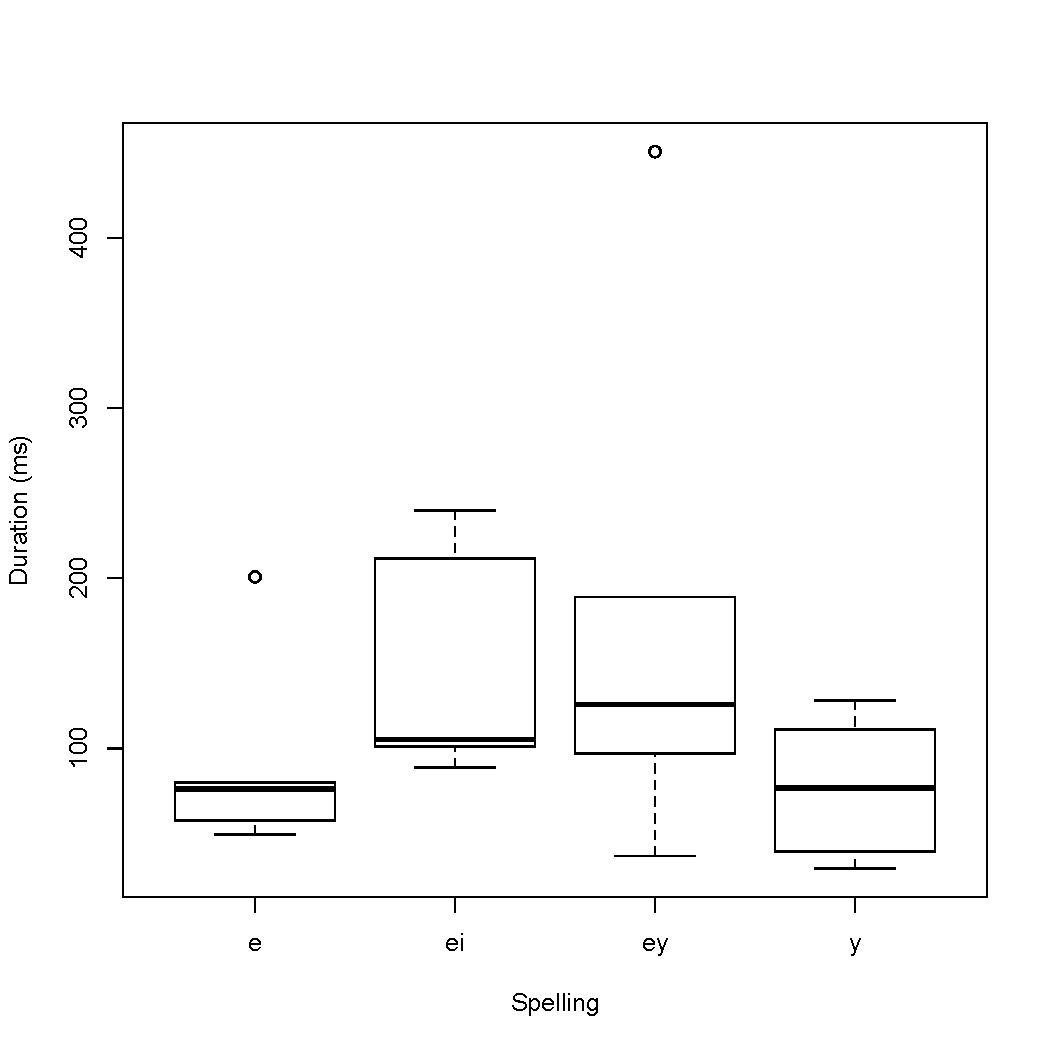
\includegraphics[width=\textwidth]{littleDur.pdf}
		\caption{Group 1}
		\label{fig:1Dur}
	\end{subfigure}
	\begin{subfigure}[b]{0.45\textwidth}
		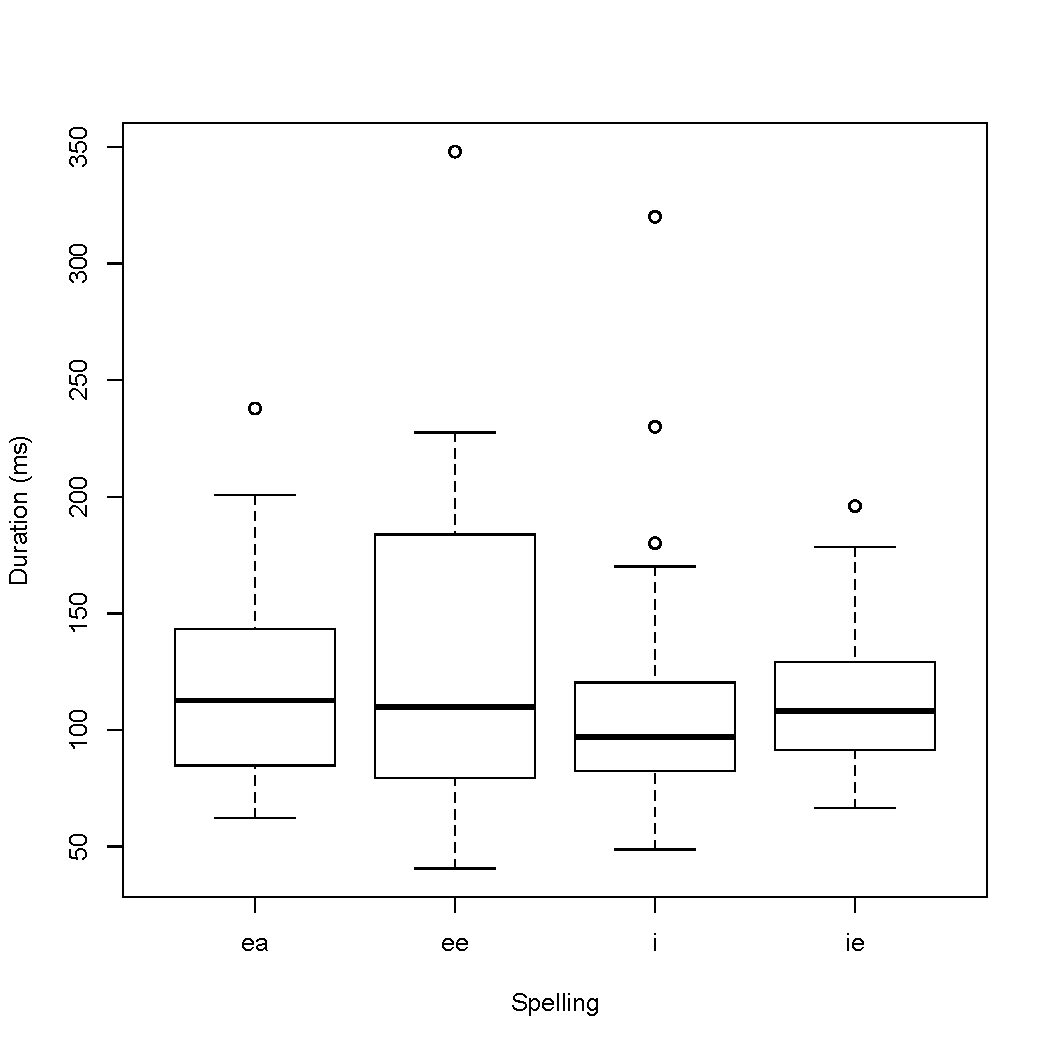
\includegraphics[width=\textwidth]{BigDur.pdf}
		\caption{Group 2}
		\label{fig:2Dur}
	\end{subfigure}
	\caption{A figure I included in my final paper for Dr. Jordan Sandoval's LING 411 Course: Topics in Phonetics and Phonology, Western Washington University, Spring 2016.}\label{fig:plot}
\end{figure}

{\LaTeX} allows you to import most major image formats (e.g. JPEG, PNG, PDF) using the \verb!graphicx! package. It's easiest if the image file is in the same folder as your .tex file, though it is possible to specify a separate folder either directly or using \verb!\graphicspath!. An example with source code is provided in Figure \ref{fig:image}, while Figure \ref{fig:plot} is more typical of something you might see in a technical linguistics paper. These specific plots were created using R Statistical Software \cite{RStats}. Note from Figure \ref{fig:imsource} the \verb![h]! option in \verb!\begin{figure}[h]!; this is used to give {\LaTeX} an idea of where you would like to position the figure. {\LaTeX} usually does a pretty good job at placing figures somewhere that minimizes blank space, but if you want more control over where the figure goes, some common options include \verb!h! (place the figure approximately here), \verb!H! (place the figure at precisely the location from the source code), \verb!t! (top of page), \verb!b! (bottom of page), or \verb!p! (put it on a special page for figures). It may take some trial-and-error to find what works best for you. Also, note the ability to place the caption at the top or bottom of the figure by placing the \verb!\caption{}! command either at the beginning or end of the \verb!figure! block, respectively. For more detailed examples, there's a fantastic wiki page on figures \url{https://en.wikibooks.org/wiki/LaTeX/Floats,\_Figures\_and\_Captions}.

Now that you've learned the basics, it's time to move on to linguistics!

\section{Phonology}
Phonetics and Phonology require a very special set of characters: the International Phonetic Alphabet (IPA). Instead of having to download a new font, put it in the proper folder on your computer, make sure it's compatible with whatever word processor you're using, and struggle to remember the shortcut keys that produce certain symbols, with {\LaTeX} you simply include \verb!\usepackage{tipa}! in your preamble. This provides all the IPA symbols you'll need in writing a phonetics or phonology paper. A useful table with all the IPA symbol encodings is provided at \url{http://people.ucsc.edu/~ajgreenw/LaTeXTIPASymbols.pdf}. As a simple example, if I type the command \verb!\textipa{DIs Iz In \t{aI} p\super hi \t{eI}! {\LaTeX} produces:
\begin{center}
\textipa{DIs Iz In \t{aI} p\super hi \t{eI}}
\end{center} 

And if you need to create columns of data, no problem! Just use the \verb!tabular! environment, where the number of columns and alignment are specified in the argument to the \verb!\begin{tabular}! command. Columns are separated by the \& character. As an example, the commands in Figure \ref{fig:data} produce the following output:

\begin{figure}[htb]
\centering
\caption{An example dataset using tabular environment}
\label{fig:data}
\begin{tabular}{c}
\begin{lstlisting}
\begin{center}
\begin{tabular}{ l l l }
\textipa{[DIs]} & \textipa{[Iz]} & \textipa{[\ae n]} \\
\textipa{[Egz\ae mp\s{l}]} & \textipa{[deR@sEt]} & \textipa{[fo\*r]} \\
\textipa{[ju]} & \textipa{[t\super hu]} & \textipa{[En\t{dZ}\t{OI}]} 
\end{tabular}
\end{center}
\end{lstlisting}

\end{tabular}
\end{figure}

\begin{center}
\begin{tabular}{ l l l }
\textipa{[DIs]} & \textipa{[Iz]} & \textipa{[\ae n]} \\
\textipa{[Egz\ae mp\s{l}]} & \textipa{[deR@sEt]} & \textipa{[fo\*r]} \\
\textipa{[ju]} & \textipa{[t\super hu]} & \textipa{[En\t{dZ}\t{OI}]} 
\end{tabular}
\end{center}

It is also possible to easily write phonological rules using the \verb!phonrule! package. A simple example and its typeset output is provided in Figure \ref{fig:rule}.

\begin{figure}[htb]
\caption{Phonological rule example commands}
\label{fig:rule}
\begin{tabular}{c}
\begin{lstlisting}
\textit{Word-final obstruent devoicing} \\
\hspace*{1cm} \phonr{\phonfeat{-sonorant \\ +voice}}
				{\phonfeat{-voice}}{\#} \\
\textit{An obstruent in word-final position will get devoiced.}
\end{lstlisting}
\end{tabular}

\vspace{15pt}

\textit{Word-final obstruent devoicing} \\
\hspace*{1cm} \phonr{\phonfeat{-sonorant \\ +voice}}
				{\phonfeat{-voice}}{\#} \\
\textit{An obstruent in word-final position will get devoiced.}
\end{figure}

With the easy-to-use commands outlined in this section, you can create beautifully organized phonetics and phonology papers with little hassle. Next, we'll look at how {\LaTeX} makes writing Syntax papers just as easy.

\section{Syntax}

A major component of Syntax papers is diagramming sentences in tree diagrams. Conveniently, {\LaTeX} provides a handy tree package called \verb!qtree!. A new tree is started using the \verb!\Tree! command. Each (sub-)tree is indicated by brackets. The root of a (sub-)tree is preceded by a period (.).  Leaf nodes, i.e. words in the sentence, are expressed by their labels. Below is a simple example with its corresponding commands in Figure \ref{fig:tree}. Pay close attention to the spaces before each closed bracket; they are required. The other formatting is merely meant to give some indication of tree structure and make the commands easier to read.

\begin{figure}[h]
\caption{Syntax tree example commands}
\label{fig:tree}
\begin{tabular}{c}
\begin{lstlisting}
\Tree[.IP [.DP [.D\1 [.D \textit{the} ]
                     [.NP [.N\1 [.N \textit{cat} ] ] ] ] ]
          [.I\1 [.I \textsc{past} ]
                [.VP [.V\1 [.V \textit{sat} ]
                           [.PP [.P\1 [.P \textit{on} ]
                                \qroof{\textit{the mat}}.DP ] ] ] ] ] ]
\end{lstlisting}
\end{tabular}
\end{figure}


\Tree[.IP 	[.DP 	[.D\1 	[.D \textit{the} ]
				[.NP 	[.N\1 	[.N \textit{cat} ] ] ] ] ]
		[.I\1	[.I \textsc{past} ]
			[.VP	[.V\1 	[.V \textit{sat} ]
					[.PP	[.P\1	[.P \textit{on} ]
							\qroof{\textit{the mat}}.DP ] ] ] ] ] ]

\clearpage

Yet for many this string of commands and brackets may be confusing and, admittedly, there are many things {\LaTeX} can't do (easily), such as tracing word movement. If you prefer to use an external tree diagram software package (e.g. TreeForm), you can save your diagram as an image and import it into your {\LaTeX} document as a figure (see Section \ref{figures}).

Another tool critical to Syntax papers is numbering glosses and examples. It's often necessary to change the order of examples many times before a paper is complete. {\LaTeX} makes this easy with the package \verb!gb4e!. (IMPORTANT: be sure to make \verb!gb4e! the last \verb!\usepackage! call in the preamble, otherwise you might get an error.) Instead of having to go back through, changing the number of each example by hand -- potentially missing one -- all you have to do is cut and paste the line \verb!\ex Example Sentence! and {\LaTeX} does the rest. Example commands and output are given below in Figure \ref{fig:nums}.

\begin{figure}[htb]
\caption{Example commands for numbered examples}
\label{fig:nums}
\begin{tabular}{c}
\begin{lstlisting}
\begin{exe}
	\ex This is an example sentence!
	\ex This sentence is grammatical English.
	\ex[*] {This sentence English in ungrammatical is.}
\end{exe}
\end{lstlisting}
\end{tabular}
\end{figure}

\begin{exe}
	\ex This is an example sentence!
	\ex This sentence is grammatical English.
	\ex[*] {This sentence English in ungrammatical is.}
\end{exe}

These tools should be enough to get you started down the path of magnificent syntax papers. For more detailed examples on numbered examples and glosses, refer to the Linguistics specific LaTeX wiki (Appendix B).

\section{End Material}
\subsection{Bibliography}
The biblography is a vital part of any research paper. It gives credit to the authors whose ideas helped shape your argument. But if you have, say, 20 references, typing out each one and making sure they're alphabetized and in the correct format can be a pain. So why not let LaTeX do the work for you? In this section, we'll see one way to add a bibliography to your document. There are many other ways, (and one of them may be more appropriate depending on your operating system or desired format) but I demonstrate this specific method because it's the easiest way I've found to get everything in APA format, which is the format most linguistics papers follow.

\begin{figure}[h]
\centering
\caption{An example BibTeX entry}
\label{fig:bibex}
\begin{tabular}{c}
\begin{lstlisting}
@Manual{RStats, % The short label to reference it by
    title = {R: A Language and Environment for Statistical Computing},
    author = {{R Development Core Team}},
    organization = {R Foundation for Statistical Computing},
    address = {Vienna, Austria},
    year = {2008},
    note = {{ISBN} 3-900051-07-0},
    url = {http://www.R-project.org},
  }
\end{lstlisting}
\end{tabular}
\end{figure}

It's possible to embed your references directly where you want the bibliography to go, but it's cleaner (and more instructive) to provide your references in a separate .bib file using what are called BibTeX entries. The benefit to using BibTeX entries is that many online journals or article databases provide a BibTeX entry for each article, which means you just have to copy+paste and let {\LaTeX} do the rest! An example BibTex entry is provided in Figure \ref{fig:bibex}. I've included several other entries in my .bib file, but because I don't actually cite them, they won't appear in my reference list. They're there to give you an idea of how to define your own BibTeX entry if the online journal, etc. doesn't provide one.

When you want to cite the article (or Software, in my case) just call \verb!\cite{<label>}! with the short label you defined in the reference's BibTeX entry. The other commands you need to know are \verb!\usepackage{apacite}!, which should go in your preamble, and \verb!\bibliographystyle{apacite} \bibliography{bibliography.bib}!, where bibliography.bib is the name of your .bib file. The last two commands should be called wherever you want your reference list to be displayed, e.g. after the appendices.

After typesetting your document, if the citations don't appear, go to the drop-down next to the typeset button, select BibTeX, hit the typeset button, then run the typeset procedure one last time with pdfLaTeX (or whatever you were using that worked).

\subsection{Appendices}
When writing a linguistics paper, you frequently have too much data to include in the main body of your text. But it's still important to include all that data so readers can replicate your experiments. That's where appendices come in. It's where you dump everything that doesn't belong in the main text but is still there for those interested. I've included two appendices for your reference. One is data from the Buckeye Corpus \cite{buckeye} that I used in LING 411 (refer back to Figure \ref{fig:plot}), and the other is a list of websites I think are useful but take up too much space when referred to in-line.

\section{Conclusion}
While it takes much longer than the few hours before a paper is due to master {\LaTeX}, we've seen how a basic grasp of specific linguistics packages such as \verb!tipa! and \verb!qtree! can make formatting easy! With the tools outlined in this paper and a few hours of practice, anyone can create beautiful linguistics papers. And we've barely scratched the surface! There's a multitude of other {\LaTeX} packages and commands you can use to make your documents even more awesome! But I'll leave those for you to discover. In the meantime, let all your words, diagrams, and fonts fall neatly in place and say goodbye to time and frustration spent herding cats.

\appendix
\section*{Appendix A: Sample Data}
The number in parentheses indicates the number of tokens considered for that word. A type without a number specified has a token count of one (1).

\linespread{1.0}\selectfont
\vspace{4ex}
\noindent
\textbf{Group 1 (6 words each):} \\
\begin{small}
\begin{tabular}{l | l | l | l }
\textbf{e} & \textbf{ei} & \textbf{ey} & \textbf{y} \\ \hline
recipe(3)  & caffeine & disney (10) & accurately \\
arena (2) & ceiling & keyboard & biology (3) \\
egotistical & protein (2) & chocolatey & ecstasy (6) \\
eon & neil & eyor & sanctuary (2)\\
cerebral & conceive (2) & parsley & agony \\
creole & deceiving & rodney & controversy \\
\end{tabular}
\end{small} \\ \\ \\
\noindent
\textbf{Group 2 (24 words each):} \\
\begin{small}
\begin{tabular}{l | l | l | l }
\small
\textbf{ee} & \textbf{ea} & \textbf{ie} & \textbf{i} \\ \hline
breed & appearances & achieve (3) & funniest \\
disagreement (2) & bean & agencies & scarier \\
dundee & beaver & apiece & vienna \\
esteem & conceal & belief (10) & assigning \\
feeble & eager & boundaries & chili \\
freeway (8) & feasible (2) & buggies & deviate \\
glee & guinea (2) & cashier & ding (4)\\
greece & ideal (5) & ceremonies (3) & gasoline (4)\\
nominee & jeans & comedies & indian (9)\\
oversee & mainstream (2) & communities (2) & ink \\
peeling & plea (5) & mommies & victoria \\
proceeded (2) & reaper & hippie & mafia (2) \\
racketeering & sears (4) & juries & mini (2) \\
reel (1) & seas & penalties (5)& missouri (4) \\
screening (6) & squealer & piercings & parochial (3)\\
sheer (2) & squeamish & policies (2) & ski (2)\\
sneeze & tease (2) & johnnie & skiing (2)\\
steer & breathed & rabies & sodium \\
tee (2) & wheat & relieve & studios \\
teen (6) & cleaver & retriever (2) & visa (4) \\
tennessee (6) & spears & spiel & committing \\
tweed & bleach & thingies & zucchini \\
unseen (3) & feature (2) & tootsie & trivia \\
yankees & leash (2) & zombie & naive (2)\\
\end{tabular}
\end{small}

\section*{Appendix B: {\LaTeX} Documentation}

\subsection*{General}
\url{https://latex-project.org/guides/} \\
\url{https://www.sharelatex.com/learn/Main_Page}\\
If you can't quickly find an answer to your question in the documentation, Google it! There are many more helpful resources available for \LaTeX.

\subsection*{Linguistics Specific}
\url{https://en.wikibooks.org/wiki/LaTeX/Linguistics} \\
IPA encodings: \url{http://people.ucsc.edu/~ajgreenw/LaTeXTIPASymbols.pdf} \\
Phonological Rules: \url{http://ctan.math.utah.edu/ctan/tex-archive/macros/latex/contrib/phonrule/phonrule-doc.pdf} \\
Qtree: \url{http://www.ling.upenn.edu/advice/latex/qtree/qtreenotes.pdf} \\
Some Style Guides and Guidelines to Writing Linguistics Papers (not {\LaTeX} specific):
\begin{itemize}
\item \url{http://www.linguisticsociety.org/sites/default/files/LANGUAGE_journal_style_sheet.pdf}
\item \url{http://www.anglistik.uni-jena.de/wp-content/pdfs/linguistik/Practical\%20Guidelines\%20for\%20Papers\%20in\%20Linguistics_2010.pdf}
\item \url{http://www.lel.ed.ac.uk/~lhlew/WritingGuidance.pdf}
\end{itemize}

\bibliographystyle{apacite}
\bibliography{ling.bib}

\end{document}
